


%\documentclass[a4paper,10pt]{article}
\documentclass[12pt]{article}
\usepackage{amsfonts}
\usepackage{graphicx}
\usepackage{amssymb}
\usepackage{amsmath}
\usepackage{longtable}
%\usepackage{color}
\usepackage{listings}
\usepackage[usenames,dvipsnames]{color}
\definecolor{MyDarkGreen}{rgb}{0.0,0.4,0.0}
%\usepackage[pdftex]{graphicx}
%\usepackage{mathtools}
\usepackage{listings}
\lstset{language=C++}
\numberwithin{equation}{section} %sets equation numbers <chapter>.<section>.<index>
%\numberwithin{equation}{subsection} %sets equation numbers <chapter>.<section>.<subsection>.<index>
%\numberwithin{equation}{subsubsection} %sets equation numbers <chapter>.<section>.<subsection>.<subsubsection>.<index>
%===================================================================================================================
% Basic Commands for Page settings,Chapters, Appendices, Sections, etc..

\setlength{\oddsidemargin}{.5in} \setlength{\topmargin}{0in}
\setlength{\headheight}{.2in} \setlength{\headsep}{.2in}
\setlength{\textwidth = 6.0in} \setlength{\textheight = 8.3in}


\def\thebiblio#1{\list
{[\arabic{enumi}]}{\settowidth\labelwidth{[#1]}\leftmargin\labelwidth
\advance\leftmargin\labelsep
\usecounter{enumi}}
\def\newblock{\hskip .11em plus .33em minus .07em}
\sloppy\clubpenalty4000\widowpenalty4000
\sfcode`\.=1000\relax}
\let\endthebiblio=\endlist

\newcommand{\sect}[1]{% Basic settings for general chapters
\cleardoublepage
\clearpage
\newpage
\begin{center}
\addtocounter{section} {1}
\setcounter{subsection} {0}
\section* {\normalsize \bf{CHAPTER \thesection \\ #1}}
\addcontentsline{toc}{section}{CHAPTER
\protect\numberline{\thesection : } #1\dotfill}
\end{center}
\thispagestyle{myheadings} }

\newcommand{\appen}[1]{% Basic settings for appendix chapters
\cleardoublepage
\clearpage
\newpage
\begin{center}
\addtocounter{section} {1}
\renewcommand{\thesection}{\Alph{section}}
\setcounter{subsection} {0}
\setcounter{table}{0}
\section* {\normalsize \bf{APPENDIX \thesection \\ #1}}
\addcontentsline{toc}{section}{APPENDIX
\protect\numberline{\thesection : } #1\dotfill}
\end{center}
\renewcommand{\thesubsection}{\Alph{section}.\arabic{subsection}}
\renewcommand{\thesubsubsection}{\Alph{section}.\arabic{subsection}.\arabic{subsubsection}}
\renewcommand{\theequation}{\Alph{section}.\arabic{equation}}
\renewcommand{\thetable}{\Alph{section}.\arabic{table}}

\thispagestyle{myheadings} }

%===================================================================================================================
% Basic Commands for Theorem, Lemma,Proposition,etc.....

\renewcommand{\baselinestretch}{2}
\renewcommand{\arraystretch}{.5}
\newcommand{\qed}{\hfill$\Box$}
\newtheorem{fact}{Theorem}[section]
\newtheorem{claim}{Claim}
\newtheorem{theorem}[fact]{Theorem}
\newtheorem{word}[fact]{Definition}
\newtheorem{prop}[fact]{Proposition}
\newtheorem{ob}[fact]{Observation}
\newtheorem{Corollary}[fact]{Corollary}
\newtheorem{corollary}[fact]{Corollary}
\newtheorem{lemma}[fact]{Lemma}
\newtheorem{Guess}[fact]{Conjecture}
\newtheorem{conj}[fact]{Conjecture}
\def\theotheorem{A\arabic{otheorem}}

\lstloadlanguages{Matlab}%
\lstset{language=Matlab,                        % Use MATLAB
        frame=single,                           % Single frame around code
        basicstyle=\small\ttfamily,             % Use small true type font
        keywordstyle=[1]\color{Blue}\bf,        % MATLAB functions bold and blue
        keywordstyle=[2]\color{Purple},         % MATLAB function arguments purple
        keywordstyle=[3]\color{Blue}\underbar,  % User functions underlined and blue
        identifierstyle=,                       % Nothing special about identifiers
                                                % Comments small dark green courier
        commentstyle=\usefont{T1}{pcr}{m}{sl}\color{MyDarkGreen}\small,
        stringstyle=\color{Purple},             % Strings are purple
        showstringspaces=false,                 % Don't put marks in string spaces
        tabsize=5,                              % 5 spaces per tab
        %
        %%% Put standard MATLAB functions not included in the default
        %%% language here
        morekeywords={xlim,ylim,var,alpha,factorial,poissrnd,normpdf,normcdf},
        %
        %%% Put MATLAB function parameters here
        morekeywords=[2]{on, off, interp},
        %
        %%% Put user defined functions here
        morekeywords=[3]{FindESS, homework_example},
        %
        morecomment=[l][\color{Blue}]{...},     % Line continuation (...) like blue comment
        numbers=left,                           % Line numbers on left
        firstnumber=1,                          % Line numbers start with line 1
        numberstyle=\tiny\color{Blue},          % Line numbers are blue
        stepnumber=5                            % Line numbers go in steps of 5
        }

% Includes a MATLAB script.
% The first parameter is the label, which also is the name of the script
%   without the .m.
% The second parameter is the optional caption.
\newcommand{\matlabscript}[2]
  {\begin{itemize}\item[]\lstinputlisting[caption=#2,label=#1]{#1.m}\end{itemize}}





\begin{document}
\pagestyle{empty}
\pagenumbering{roman}

%================================================ Title Page ======================================================
\begin{center}
{THESIS TITLE MTSU MATHEMATICAL  \\
[.10in]
 SCIENCES DEPARTMENT THESIS FORMAT  \\ [.07in]} \rm
\rule{1.25in}{.01in}\\[.0 in]

\vspace{.6in}

A Thesis \\ [.06  in]
Presented to the Faculty of the  Department of Mathematical Sciences \\[.06in]
Middle Tennessee State University \\ [.06in]
\rule{1.25in}{.01in}\\

\vspace{.6in}

In Partial Fulfillment \\[.06 in]
of the Requirements for the Degree \\ [.06 in]
Master of Science in Mathematical Sciences \\ [.06 in]
\rule{1.25in}{.01in}\\

\vspace{.6in}

by  \\ [.06in]
{ Name of Author} \\[.06in]
{August 2012}
\end{center}

%================================================ Approval Page ===================================================
\newpage

\pagestyle{plain}

\begin{center}

{\bf APPROVAL} \\ [.05in]
{\bf This is to certify that the Graduate Committee of }\\
Name of Author \\ [-.1in] met on the \\ [-.1in] 1st \  day of \
August, 2012.
\\ [.25in]
\end{center}

\baselineskip=20 pt

 The committee read and examined his/her thesis,
supervised his/her defense of it in an oral examination, and decided
to recommend that his/her study should be submitted to the Graduate
Council, in partial fulfillment of the requirements for the  degree
of Master of Science in Mathematics.

\vspace{.3in}

\noindent
\makebox[3.4in][l]{}\makebox[2.0in][l]{\rule{2.5in}{.01in}}\\[-.1in]
\makebox[3.4in][l]{} \makebox[2.0in][l]{\it Dr. A.Q.M.Khaliq}\\[-.1in]
\makebox[3.4in][l]{} \makebox[2.0in][l]{Chair, Graduate Committee } \\[.1in]
\makebox[3.4in][l]{} \makebox[2.0in][l]{\rule{2.5in}{.01in}} \\[-.1in]
\makebox[3.4in][l]{} \makebox[2.0in][l]{\it Dr. Zachariah Sinkala} \\[.1in]
\makebox[3.4in][l]{} \makebox[2.0in][l]{\rule{2.5in}{.01in}} \\[-.1in]
\makebox[3.4in][l]{} \makebox[2.0in][l]{\it Dr. Yuri Melnikov} \\[.1in]
\makebox[3.4in][l]{} \makebox[2.0in][l]{\rule{2.5in}{.01in}} \\[-.1in]
\makebox[3.4in][l]{} \makebox[2.0in][l]{\it Dr. James Hart} \\[-.1in]
\makebox[3.4in][l]{}\makebox[2.0in][l]{ Graduate Coordinator,} \\[-.1in]
\makebox[3.4in][l]{}\makebox[2.0in][l]{ Department of Mathematical Sciences} \\[.1in]
\makebox[3.4in][l]{} \makebox[2.0in][l]{\rule{2.5in}{.01in}} \\[-.1in]
\makebox[3.4in][l]{} \makebox[2.0in][l]{\it Dr. Don Nelson} \\[-.1in]
\makebox[3.4in][l]{}\makebox[2.0in][l]{ Chair,} \\[-.1in]
\makebox[3.4in][l]{}\makebox[2.0in][l]{ Department of Mathematical Sciences} \\[.1in]
\makebox[3.4in][l]{Signed on behalf of } \makebox[2.0in][l] {\rule{2.5in}{.01in}}\\[-.1in]
\makebox[3.4in][l]{the Graduate Council}\makebox[2.0in][l]{\it Dr. Michael Allen} \\[-.1in]
\makebox[3.4in][l]{}\makebox[2.0in][l]{ Dean,} \\[-.1in]
\makebox[3.4in][l]{}\makebox[2.0in][l]{ School of Graduate Studies}

%================================================ Abstract Page =================================================

\newpage
\begin{center}
{\bf ABSTRACT}\\
\end{center}
\baselineskip=24pt


Meshfree radial basis functions (RBF) is an interpolation technique
for constructing an unknown function from scattered data. In this
thesis we apply an efficient RBF method in evaluating the price of
standard European and American options. The analytical solution of
the European option exists and can be obtained by the Black-Scholes
formula. There is no exact solution of the American option problem
due to the existence of an early exercise constraint which leads to
a free boundary condition. We evaluate the American Option by adding
a small continuous nonlinear penalty term to the Black-Scholes model
to remove the free boundary condition. The application of RBFs leads
to a system differential equations which are solved by a time
integration scheme known as the $\theta$-method.The option price is
approximated with RBF with unknown parameters at each time step. We
compare the accuracy, efficiency and computation cost of three RBFs
Gaussian, Multiquadric and the Inverse-multiquadric.Finally a
comparison is made between the three RBFs and the solution obtained
by finite difference.\mathbb{R}


%================================================ Copyright Page =================================================
\newpage
\baselineskip=24 pt
\begin{center}
\ \ \
\vspace{3.in}

Copyright \copyright\ 2012, Nana Akwasi Abayie Boateng
\end{center}


%================================================ Dedication Page =================================================
\newpage

\begin{center}

{ \bf DEDICATION } \\ [.15in]
\end{center}

This thesis is dedicated to my parents, who has taught me,
encouraged me and supported me in my life. Thanks for all your
patience, love and unconditional support.


%================================================ Acknowledgments Page ==============================================
\newpage
\begin{center}

{ \bf ACKNOWLEDGMENTS} \\ [.15in]
\end{center}

Take this opportunity to thank your advisor, your thesis committee,
research collaborators and anyone who helped you in the process of
thesis accomplishment.




%================================================ Table of Content  =================================================
\newpage

\tableofcontents
%%================================================ Chapter 1 ==============================================================
%{INTRODUCTION}
%%================================================ Chapter 2 ==============================================================
%{\uppercase{Option Pricing}}
%%--
%%================================================ Chapter 3 ==============================================================
%\uppercase{Finite Difference Methods}\\
%%-------------------------------------------------------------------------------------------------------------------------
%%================================================ Chapter 4 ==============================================================
%\uppercase{RBF-Meshfree Methods}\\
%%-------------------------------------------------------------------------------------------------------------------------
%
%%================================================ Chapter 5 ==============================================================
%\uppercase{Discretization And Algorithms}\\
%%-------------------------------------------------------------------------------------------------------------------------
%%================================================ Chapter 7 ==============================================================
%\uppercase{ Numerical Methods and  Stability Analysis }\\
%%================================================ List of Tables  ===================================================

%%================================================ Chapter 6 ==============================================================
%\uppercase{Numerical Experiments And Results}\\
%%-------------------------------------------------------------------------------------------------------------------------

\newpage
\addcontentsline{toc}{section}{\rm LIST OF TABLES}
\listoftables



%================================================ List of Figures ====================================================
\newpage
\addcontentsline{toc}{section}{\rm LIST OF FIGURES}
\listoffigures



\def\R{\mathbb{R}}
\def\N{\mathbb{N}}
\def\Z{\mathbb{Z}}
\def\Q{\mathbb{Q}}
\def\la{\langle}
\def\ra{\rangle}

\def\dist{{\rm dist}}
\def\X{{\bf X}}
\def\C{{\bf C}}
\def\D{{\bf D}}
\def\I{{\bf I}}
\def\J{{\bf J}}
\def\x{{\bf x}}
\def\y{{\bf y}}
\def\z{{\bf z}}
\def\W{{\bf W}}
\def\g{{\bf g}}
\def\e{{\bf e}}
\def\b{{\bf b}}
\def\u{{\bf u}}
\def\Beta{{\bf \beta}}
\def\pen{{\rm pen}}
\def\argmin{{\rm argmin}}
\def\diag{{\rm diag}}
\def\sgn{{\rm sgn}}
\def\supp{{\rm\rm supp}}


\vspace*{1cm}
%============================================= Appendix Separation Page  ===============================================
\newcommand{\Appendixpage}{
    \setcounter{section}{0}
    \renewcommand{\baselinestretch}{1}\small\normalsize
    \thispagestyle{myheadings}
    \addcontentsline{toc}{section}{APPENDICES\dotfill}
    \mbox{}
    \vfil
    \begin{center}%
    APPENDICES
    \vfil
    \end{center}%
    \renewcommand{\baselinestretch}{1.66} \small\normalsize%
    \cleardoublepage
  }

%================================================ Chapter 1 ==============================================================
\sect{INTRODUCTION}
\pagestyle{myheadings} \markboth{  } {  }
\pagenumbering{arabic}
%-------------------------------------------------------------------------------------------------------------------------
An option is a financial contract which gives the holder of the
option the right to purchase or sell a prescribed asset at a
prescribed time in the future known as the expiry date at a
prescribed amount which the exercise or strike price.

In 1973,Fisher Black and Myron Scholes showed that the option value
of the European call option can be modeled by a lognormal diffusion
partial differential equation.There are two categories of options
namely, standard options(European and American options) and non
standard options.
 Hon and Mao\cite{Hon} introduced a numerical scheme in which by
 applying global radial basis function as a spatial approximation
 for the numerical solution of the value of the  value of the option
 and it's derivative in the Black-Scholes equation.From their
 numerical results,they showed that the use of RBFs does not require
 the generation of a rectangular grid and also the computational
 domain is composed of scattered data points.
 Khaliq \textit{et al}\cite{KK} investigated meshfree RBF approximation to
 options with non-smooth payouts.By taking advantage of parallel
 architecture,they developed a strongly stable time stepping fourth
 order method which was a linear combination of four Backward
 Euler-like solver on four concurrent processors.
 Khaliq \textit{et al}\cite{ADS06} considered a penalty method
 approach to solving  American options.They observed that by
 introducing a carefully chosen continuous penalty term to the
 Black-Scholes equation,the free and moving boundary condition can
 be removed and allow the problem to be solved on a fixed
 domain.They introduced a linearly implicit scheme with superior
 accuracy and stability by solving the nonlinear term explicitly.
 The remaining chapters of this thesis is organized  as follows.
 We introduce option pricing and discuss two standard option,
 the European and American options in chapter 2.In chapter 3 we adopt an Exponential
 Time Differencing version of the Backward Euler finite difference
  scheme to evaluate the price of the option. The theory and development of RBF
  Meshfree methods are presented in chapter 4.In chapter 5, we elaborate on the
  discretization and algorithms of the methods. The stability analysis and the
  results of the numerical experiments are presented in chapters 6 and 7.
  Finally all results are discussed and interpreted in chapter 7.

\subsection{Sample Section} This is a sample section.

The study of algebraic structures using its associate graphs is a
very exciting field which generates many fascinating results,
conjectures and questions \cite{Abdollahi2006}. There are various
ways to associate graphs to algebraic objects such as groups and
rings. For instance, the prime graph defined in\cite{Williams1981},
the conjugacy class graph defined in\cite{Bertram}, the
non-commuting graph defined in\cite{Abdollahi2006}, and the nonzero
divisor graph defined in\cite{DavidAnderson}

%\subsubsection{Sample Sub Section}
%This is a sample equation.
%\begin{align}
%    \frac{\partial}{{\partial}t}\int\int\limits_{system}
%                 (V_{A_{r}} + V_{A_{s}})dxdy = 0        \label{eq: equation1}\\
%    \frac{\partial}{{\partial}t}\int\int\limits_{system} V_B dxdy = 0
%                                                            \label{eq:equation2}
%\end{align}
%\begin{theorem}{\rm(\cite{Wang2008})}\label{thm1}
%Let $G$ be a group such that $\nabla{(G)} \cong\nabla(A_{n})$, where
%$n\ge 5$. If $n=5,6$ or at least one of $n,n-1,n-2$ is prime then
%$G\cong A_{n}$.
%\end{theorem}
%================================================ Chapter 2 ==============================================================
\sect{\uppercase{Option Pricing}}
% \numberwithin{Option Pricing}
%-------------------------------------------------------------------------------------------------------------------------

%\subsection{What is an Option?}

An option is a financial contract which gives the holder of the
option the right to purchase  or sell a prescribed asset at a
prescribed time in the future known as the expiry date at a
prescribed amount which the exercise or strike price\cite{Wilmot}.
 The most common kinds of prescribed assets which are traded on
financial markets are stocks,bonds,currency and commodities.An
option is a derivative product because it is traded on an underlying
asset.The holder of a call option makes profit if the price of the
underlying asset rises on the market whereas the holder of a put
option does so when the price of the underlying asset falls on the
financial market.The two primary uses of option are for hedging and
speculation\cite{Wilmot}.
 There are numerous kinds of options which are
traded on financial markets.Vanilla options are options  which  do
not possess any special features or characteristics.Examples are the
European and American options.Exotic options possess special
features.Examples include Asian options,Barrier options,Basket
options.In this We consider The  European and American options.




%\subsubsection{The European Options}
\subsection{The European Options}
%\numberwithin{equation}{The European Options}
 The European option is an option
which can only be exercised at its maturity time.The exact or
analytical formula for estimating a fair price   for European
options exist. In 1973 Black and Scholes by making  a set of
explicit  assumptions including  the risk-neutrality of the
underlying asset price showed that the value European  call option
satisfies a backward -in-time lognormal partial differential
equation of diffusion type which has come to be known as the
Black-Scholes equation\cite{BS73}.
  Let the $V(S,t)$ be the price of an option which is function of both
  asset price and time.This option satisfies the following
  Black-Scholes equation.
  \begin{equation} \label{BSS}
\frac{\partial P}{\partial t}+\frac{1}{2}\sigma^2S^2\frac{\partial^2
P}{\partial S^2} +rS\frac{\partial P}{\partial S}-rP=0, \quad S
> \overline{S}(t),\ 0 \le t < T.
\end{equation}
where $r$ is the risk-free interest interest rate,$\sigma$ is the
volatility of the asset price,$S$ is the asset price.The Final
condition is given by\cite{Wilmot}
\[V(S,t) = \left\{
\begin{array}{l l}\label{FNC}
  max\{E-X,0\} & \quad \mbox{ for a put option}\\
  max\{S-E,0\}& \quad \mbox{for a call option}\\ \end{array} \right. \]
  where E is the strike price.\\
  The Boundary condition  of the European call option  is given as
  follows:
  \begin{equation}
C(S,t)\thicksim S  \quad
 as S\rightarrow\infty ,\quad C(0,t)=0.
\end{equation}
where $C(S,t)$ is the value of the European call option satisfying
\ref{BSS}. The Boundary condition  at of the European put option is
given as follows:
% \begin{equation}\label{FC}
%P(S,t)\rightarrow 0 as S\rightarrow\infty  \quad as ,\quad
%P(0,t)=E\exp^{\int^{T}_{t}\tau(\tau)d\tau}}.
%\end{equation}
where $P(S,t)$ is the value of the European put  option
satisfying equation \ref{BSS} for a time dependent interest rate.\\
 Equation \ref{BSS} can be transformed exponentially by making the
substitution $S=e^y$ to

 \begin{equation}
\frac{\partial U}{\partial
t}+\frac{1}{2}\sigma^2\frac{\partial^2U}{\partial
y^2}+(r-\frac{1}{2}\sigma^2\frac{\partial U}{\partial y})-rU=0
\end{equation}

\[U(y,T) = \left\{
\begin{array}{l l}\label{INC}
  max\{E-e^y,0\} & \quad \mbox{ for a put option}\\
  max\{e^y-E,0\}& \quad \mbox{for a call option}\\ \end{array} \right. \]
The analytical solution of the Black- Scholes partial differential
equation \ref{BSS} with corresponding final and initial conditions
\ref{FNC} and \ref{FC} with a constant volatility and interest rate
 for the European call option is given as\cite{Wilmot}
\begin{equation}
C(S,t)=SN(d_1)-E\exp^{-r(T-t)}N(d_2)
\end{equation}
where $N(.)$ is the cumulative  distribution function for the
standardized normal random variable given by
\begin{equation}
N(x)=\frac{1}{\sqrt{2\pi}}\int^{x}_{-\infty}\exp^{-\frac{1}{2}y^2dy}
\end{equation}
The corresponding analytical solution of the European put option is
given by
\begin{equation}
P(S,t)=E\exp^{-r(T-t)}N(-d_2)-SN(-d_1)
\end{equation}


where\\
\begin{equation*}
d_1=\frac{\log(\frac{S}{E}+(r+\frac{1}{2}\sigma^2)(T-t))}{\sigma\sqrt{T-t}}
\end{equation*}
\begin{equation*}
d_2=\frac{\log(\frac{S}{E}+(r-\frac{1}{2}\sigma^2)(T-t))}{\sigma\sqrt{T-t}}
\end{equation*}

\begin{figure}[h]
\begin{centering}
\vskip -0.5in
\includegraphics*[height=3in]{calloption.png}\
\caption{The pay-off of the European Call Option }
\includegraphics*[height=3in]{putoption2.png}\
\caption{The pay-off of the European Put Option } \vskip -0.5in
\end{centering}
\end{figure}

%\subsubsection{The American Option}
\subsection{The American Options}
The American option can be exercised at any time prior to expiry.The
American option is complicated because at at each time $t$ not only
is one interested in the value of the option but also for each asset
price $S$,whether it should be exercised or not.This creates a free
boundary problem\cite{Wilmot}.At each time $t$ there is a particular
value of $S$ which lies in the boundary between two regions:one
where early exercise is optimal to the other where one should hold
on to the option.The optimal exercise price$s_{f}(t)$ which in
general depends on time is not known \textit{priori} unlike the case
of European options.The American option valuation can be uniquely
specified by a set of constraints among which are the option value
must be greater than or equal to the payoff function, the option
value must be continuous function of $S$,replacing the Black-Scholes
equation by an inequality and lastly making the derivative of the
option with respect to the asset price(option delta) continuous.
 The value $V(S,t)$ of the American option satisfies the following
 inequality
 \begin{equation}
\frac{\partial V}{\partial t}+\frac{1}{2}\sigma^2S^2\frac{\partial^2
V}{\partial S^2} +rS\frac{\partial V}{\partial S}-rV\leq 0
 \end{equation}

The Final condition is at expiry time $T$ given by\cite{Wilmot}
\[V(S,t) = \left\{
\begin{array}{l l}\label{FNC}
  max\{E-X,0\} & \quad \mbox{ for a put option}\\
  max\{S-E,0\}& \quad \mbox{for a call option}\\ \end{array} \right. \]
  where E is the strike price.\\
  In the region$0\leq S\leq S_{f}(t)$ where early exercise is optimal,the value of the
  American put option satisfies the following inequality
 \begin{equation}
\frac{\partial P}{\partial t}+\frac{1}{2}\sigma^2S^2\frac{\partial^2
P}{\partial S^2} +rS\frac{\partial P}{\partial S}-rP< 0
 \end{equation}
 and
  \begin{equation}
P=E-S
 \end{equation}

In the other region,$S_{f}(t)< S<\infty$,early exercise is not
optimal and the value of the American put option satisfies the
Black-Scholes equation
 \begin{equation}
\frac{\partial P}{\partial t}+\frac{1}{2}\sigma^2S^2\frac{\partial^2
P}{\partial S^2} +rS\frac{\partial P}{\partial S}-rP= 0
 \end{equation}
 and
  \begin{equation}
P>E-S
 \end{equation}
 The boundary condition at$S_{f}(t)= S$ are that $P$ and its
 slope(delta) are continuous.

 \begin{equation}\label{pp}
P(S_{f}(t),t)=max(E-S_{f}(t),0)
 \end{equation}

\begin{equation}\label{dv}
 \frac{\partial P}{\partial S}(S_{f}(t),t)=-1
 \end{equation}
  The boundary condition \ref{pp} determines the option value at the
  free boundary,whereas \ref{dv}known as the \textit{smooth pasting condition} determines the location of the
  free boundary and simultaneously maximizes the benefit to the
  holder whiles avoiding arbitrage.
  The value $C(S,t)$ of the American Call  option satisfies the
  corresponding equality in the holding region
 $0\leq S\leq S_{f}(t)$
 \begin{equation}
\frac{\partial C}{\partial t}+\frac{1}{2}\sigma^2S^2\frac{\partial^2
C}{\partial S^2} +rS\frac{\partial C}{\partial S}-rC=0
 \end{equation}

in the other region where early exercise is optimal $S_{f}(t)<
S<\infty$,the value $C(S,t)$ of the American call option satisfies
 \begin{equation}
\frac{\partial C}{\partial t}+\frac{1}{2}\sigma^2S^2\frac{\partial^2
C}{\partial S^2} +rS\frac{\partial C}{\partial S}-rC<0
 \end{equation}
 and
 \begin{equation}
P=E-S
 \end{equation}
\subsection{Penalty Method}
 %An elegant transformation of this moving boundary
%problem to one on a fixed domain was suggested in \cite{ZFV98} and
%later refined in \cite{NST02}.
We  introduce a penalty term into the Black-Scholes equation, to
obtain a parabolic nonlinear partial differential equation of the
form.The introduction of the penalty term changes the problem from
that of a constrained optimization problem to that of a series of
unconstrained optimization problem.The  solution of the
unconstrained optimization problems converges to the original
constrained optimization problem.\cite{BOA08}
\begin{equation}\label{BSpenalty}
\frac{\partial P_\epsilon}{\partial
t}+\frac{1}{2}\sigma^2S^2\frac{\partial^2 P_\epsilon}{\partial S^2}
+rS\frac{\partial P_\epsilon}{\partial
S}-rP_\epsilon+\frac{_\epsilon C }{P_\epsilon + \epsilon - q(S)}=0,
\quad 0 \leq S \leq S_\infty, \ 0 \leq t < T.
\end{equation}
Here $0 < \epsilon \ll1$ is a small regularization parameter, $C
\geq rE$ is a positive constant, and $q(S) = E - S$ is the barrier
function. The value $S_\infty$ is a (relatively very large) price
for which the option is worthless. The  following are  terminal and
boundary conditions which  accompany the nonlinear nonlinear partial
differential equation.
\begin{eqnarray}
P_\epsilon(S,T) & = & \max (E-S,0)\\
P_\epsilon(0,t) & = & E,\\
P_\epsilon(S_\infty,t) & = & 0.
\end{eqnarray}
%\begin{theorem}{\rm(\cite{Wang2008})}\label{thm1}
%Let $G$ be a group such that $\nabla{(G)} \cong\nabla(A_{n})$, where
%$n\ge 5$. If $n=5,6$ or at least one of $n,n-1,n-2$ is prime then
%$G\cong A_{n}$.
%\end{theorem}





%================================================ Chapter 3 ==============================================================
\sect{\uppercase{Finite Difference Methods}}
\subsection{Finite Difference Approximations}
 The method  of Finite Difference Approximation which is based on Taylor series expansions
of functions near the point of interest will be used to discretize
the Black-Scholes partial differential equation\cite{Wilmot}
\begin{equation}
\frac{\partial P}{\partial t}+\frac{1}{2}\sigma^2
S^2\frac{\partial^2 P}{\partial ^2}+rS\frac{\partial P}{\partial
S}-rP +\frac{_{\epsilon}C}{P_{\epsilon}+\epsilon-q(s)}
\end{equation}
 The first order partial derivative $\frac{\partial P}{\partial S}$ is approximated by central differencing
 with spatial step size $h$=$\frac{S_{f}-S_{0}}{N}$ and time step size$k$=$\frac{T_{f}-T_{0}}{M}$ as
 follows.We apply the ETD-BE scheme  performing  a Backward-Euler approximation on
 $\frac{\partial P}{\partial t}$ treat the penalty$Q$ term explicitly.
 \begin{equation*}
\frac{\partial P^2}{\partial
S^2}=\frac{P_{i+1,j}-2P_{i,j}+P_{i-1,j}}{h^2}
 \end{equation*}
 \vspace{10mm}
  \begin{equation*}
\frac{\partial P}{\partial S}=\frac{P_{i+1,j}-P_{i-1,j}}{2h}
 \end{equation*}



 Using the approximations above ,the Black-Scholes partial differential
 equation is then applied to mesh points $(nk,mk)$ ,$n=1,2...N-1$,at
 the time level $t=mk$,$m=1,2,...,M$.At each $n$ we have
 \begin{equation*}
  \frac{P_{i,j}-P_{i,j-1}}{k}=\frac{1}{2}\sigma^2S^2\left[\frac{P_{i+1,j}-2P_{i,j}+P_{i-1,j}}{h^2}\right]+rs\left[\frac{P_{i+1,j}-P_{i-1,j}}{2h}\right]-rP_{i,j}+\frac{_{\epsilon}C}{P_{\epsilon}+\epsilon-q(s)}
 \end{equation*}

  \begin{equation*}
P_{i,j}-P_{i,j-1}=\frac{1}{2}\frac{\sigma^2S^2k}{h^2}\left[
P_{i+1,j}-2P_{i,j}+P_{i-1,j}\right]+\frac{krS}{2h}\left[
P_{i+1,j}-P_{i-1,j}\right]-rkP_{i,j}+\frac{_{\epsilon}Ck}{P_{\epsilon}+\epsilon-q(s)}
 \end{equation*}
 Let $\beta=\frac{1}{2}\frac{\sigma^2S^2k}{h^2}$ , $\frac{krS}{2h}$
 and $Q=\frac{_{\epsilon}Ck}{P_{\epsilon}+\epsilon-q(s)}$

 \begin{equation*}
P_{i,j}-P_{i,j-1}=\beta P_{i+1,j}-2\beta P_{i,j}+\beta
P_{i-1,j}+\alpha P_{i+1,j}-\alpha P_{i-1,j}-rkp_{i,j} +Q
 \end{equation*}

  \begin{equation*}
P_{i,j}+2\beta P_{i,j}+rkP_{i,j}-\beta P_{i+1,j}-\alpha
P_{i-1,j}-\beta P_{i-1,j}=P_{i,j-1}+Q
 \end{equation*}

 \begin{equation*}
(1+2\beta
+rk)P_{i,j}-(\alpha+\beta)P_{i+1,j}+(\alpha-\beta)P_{i-1,j}=P_{i,j-1}+Q
 \end{equation*}

This leads to the following tridiagonal system
\[A = \left( \begin{array}{cccc}
1+2\beta +rk& -(\alpha+\beta) & ...& 0\\
\alpha-\beta & 1+2\beta +rk &  & \\
& \ddots & \ddots &  \\
& & &  \\
%0 &...&\alpha-\beta & 1+2\beta +rk &-(\alpha+\beta)\\
 0&......& \alpha-\beta&1+2\beta+rk  -(\alpha+\beta) \\
 0 &...&\alpha-\beta & 1+2\beta
+rk \end{array} \right) .\] The boundary condition vector
$\textbf{b}_j$ is given by
\begin{equation*}
\textbf{b}_j=  \left[
(\alpha-\beta)P_{1},0,.......0,-(\alpha+\beta)P_{N,}\right]^{T}
 \end{equation*}

 \begin{equation*}
 AV_{i,j} + b_{j}=V_{i,j-1}+Q
 \end{equation*}
The eigenvalues of the matrix A can be shown to
%\begin{equation*}
% \begin{array}
%
% \lambda_{s}&=&1+2\beta+rk+2\sqrt{-(\alpha+\beta)(\alpha-\beta)}\cos\frac{S\pi}{N+1}
%
% \end{array}
% \end{equation*}
\begin{equation*}
\begin{array}{lcl} \lambda_{s} & = &1+2\beta+rk+2\sqrt{-(\alpha+\beta)(\alpha-\beta)}\cos\frac{S\pi}{N+1}  \\ S & = & 1\cdots N-1 \end{array}
\end{equation*}
\begin{equation*}
\lambda_s=1+2\beta+rk+2\sqrt{\beta^2-\alpha^2}\cos\frac{S\pi}{N+1}
\end{equation*}
If $0<\alpha \leq \beta$ then the eigenvalues are real numbers
satisfying
\begin{equation*}
-(1+2\beta+rk+2\sqrt{\beta^2-\alpha^2})\leq \lambda_s \leq
1+2\beta+rk+2\sqrt{\beta^2-\alpha^2}
\end{equation*}
If $\beta \leq \alpha$,then the eigenvalues are complex numbers
satisfying
\begin{equation*}
\begin{array}{cccllllc}

\lambda_s&=&1+2\beta+rk+2\sqrt{-(-\beta^2-\alpha^2)}\\
&=&1+2\beta+rk+2\sqrt{\alpha^2-\beta^2}i\\
&=&1+2\beta+rk+2i\gamma_j\\
\end{array}
\end{equation*}

where
\begin{equation*}
-\sqrt{\alpha^2-\beta^2}\leq \gamma_j\leq\sqrt{\alpha^2-\beta^2}
\end{equation*}
The eigenvalues of \textbf{A} are essential in determining the
stability of the numerical scheme above.The system is stable if
$max|\lambda_s | \leq 1$ for $S=1...N-1$
\subsection{Time Stepping Scheme}
We Consider the following nonlinear parabolic
initial-boundary value problem:
\begin{eqnarray}\label{tms1}
u_t + A u &=& F(t,u) \qquad \textrm {in} \; \Omega,\qquad t \in \left( 0,T \,\, \right], \label{Eq1}\\
u &=& v \qquad \qquad \; \, \textrm {on} \;\partial \Omega,\quad t \in \left( 0,T \,\, \right], \nonumber \\
u(\cdot,0) &=& u_0 \qquad \qquad \textrm {in} \;\Omega, \nonumber
\end{eqnarray}
where $\omega$ is a bounded domain in $\mathbb{R}^{d}$ which also
has Lipschitz continuous boundary,we let $A$ represents a uniformly
elliptic operator, and $F$ is a sufficiently smooth, nonlinear
reaction term. We represent a differential operator as follows:

\begin{eqnarray}
A := -\sum_{j,k=1}^d \frac{\partial}{\partial x_{j}} \left (
a_{j,k}(x)\frac{\partial}{\partial x_{k}} \right )+\sum_{j=1}^d
b_{j}(x)\frac{\partial}{\partial x_{j}}+b_{0}(x),
\end{eqnarray}
where the coefficients $a_{j,k}$ and $b_{j}$ are $C^{\infty}$ (or
sufficiently smooth) functions on $\overline{\Omega}$,
$a_{j,k}=a_{k,j}$, $b_{0} \ge 0$, and for some $c_0 > 0$
%\begin{eqnarray*}
% \sum_{j,k=1}^{d}a_{j,k}(\cdot)\xi_j\xi_k \geq
%c_0 \mid \xi \mid^2$,\hspace{5mm}on $\={\Omega},\hspace{5mm}for all
%\xi \epsilon\Re^d
%\end{eqnarray*}

\begin{eqnarray}
\sum_{j,k=1}^d a_{j,k}(\cdot) \xi_{j} \xi_{k} \geq c_{0}
|\xi|^2,\quad \rm on \; \overline{\Omega}, \quad \rm{for\; all} \;
\xi \in  \mathbb{R}^{d}.
\end{eqnarray}


We chose $A$ and $F$ based on an abstract formulation for
convenience to facilitate the  development of the numerical scheme
and its analysis. The initial value problem \ref{tms1} is reset to
be posed in a Hilbert space ${X}$, as follows. Consider now $A$ to
be a linear, self-adjoint, positive definite, closed operator with a
compact inverse, defined on a dense domain $D(A) \subset {X}$.  The
operator $A$ could represent  any of $\{A_h\}_{0< h \le h_0}$,
obtained through spatial discretization, and  ${X}$ We assume the
resolvent set $\rho(A)$ satisfies, for some $\alpha \in
(0,\frac{\pi}{2} )$, $\rho(A) \supset \overline{\Sigma}_{\alpha},
\,\, $ where $\Sigma_{\alpha}:= { z \in := \alpha < |\arg(z)| \leq
\pi,z \neq 0}$. Also,  assume there exists $M \geq 1$ such that
\begin{equation}
\|(zI-A)^{-1}\| \geq M |z|^{-1}, \: z \in \Sigma_\alpha.
%\label{assumption1}
\end{equation}
It follows that $-A$ is the infinitesimal generator of an analytic
semigroup $\{e^{-tA}\}_{t\ge 0}$ which is the solution operator for
\ref{tms1}, and $|e^{-tA}| \leq C$ for ${t \ge 0}$. Also, we assume
that $F(t,u(t))$ is Lipschitz on $[0,T] \times X$, i.e. it satisfies
the following assumption:

\textbf{Assumption1}
 \label{assumption2}
  \emph{ $F:[0,T] \times X
\rightarrow X$ and $U$ be an open subset of $[0,T] \times X$. For
every $(t,x) \in U$ there exists a neighborhood $V \subset U$ and a
real number $L_{T}$ such that}
\begin{eqnarray}
\|F(t_1,x_1) - F(t_2,x_2)\| \leq L_{T} ( |t_1-t_2| + \|x_1-x_2\|X)
\label{lipschitz}
\end{eqnarray}
for all $(t_i, x_i) \in V $. Using the standard representation:
\begin{equation*}
E(t) := e^{-tA} = \frac{1}{2\pi i}
\int_{\Gamma}e^{-tz}(zI-A)^{-1}dz, \label{Eq3}
 \end{equation*}
 where
 \begin{equation*}
 \Gamma := {z \in :\arg(z) = \theta}
 \end{equation*}
 , oriented so that
$\mbox{\rm Im}(z)$ decreases, for any

$\theta \in (\alpha, \frac{\pi}{2})$ and the Duhamel principle, the
exact solution  can be written as

\begin{equation}
u(t)=E(t)v+\int_{0}^t E(t-s) F(s,u(s)) ds. \label{NL-DP}
\end{equation}
Let $0 < k \le k_0$, for some $k_0$, and $t_n = nk$, $0\leq n \leq N
$. Replacing $t$ by $t+k$, using basic properties of $E$ and by the
change of variable $s-t=k\tau$,  we arrive at the following
recurrence formula for the exact solution:
\begin{equation}
u(t_{n+1})= e^{-kA}u(t_n) + k\,\int_{0}^1 e^{-kA(1-\tau)} F(t_n+\tau
k, u(t_n+\tau k))\,d\tau.\label{Ch7-Eq2}
\end{equation}
This underlines the  basis for deriving ETD schemes.
 {\em The ETD-BE Scheme}.
Denoting the semidiscrete  approximation to $u(t_n)$ by $u_n$ (note
that only the time-variable is discretized) and $F(t_n, u_n)$ by
$F_n$, the simplest approximation to the integral is to impose that
$F$ is constant for $t \in [t_n, t_{n+1}]$, i.e. $F \approx F_n$.
This yields (from (22))
\begin{eqnarray}
u(t_{n+1}) &\approx & e^{-kA}u(t_n) + e^{-kA} k  \,\int_{0}^1
e^{kA\tau} \,d\tau \,F_n \, = \, e^{-kA}u(t_n) - A^{-1}
\left(e^{-kA} - I\right) \,F_n.  \label{ETD1_sd}
\end{eqnarray}
This semidiscrete scheme becomes useful after discretization of the
matrix exponentially is efficient.Observe that


\begin{eqnarray}
 -A^{-1} \big( e^{-kA} -I \big) &=& -A^{-1}  \big(  \, (I+kA)^{-1} -I \big)\nonumber\\
             &=& -A^{-1}  \big( I-(I+kA) \,\big)(I+kA)^{-1}\nonumber\\
             &=& k \, (I+kA)^{-1}\nonumber\\
             &=& kR_{0,1}\big(kA\big),\label{derivation_ETD1}
\end{eqnarray}

this results in  a fully discrete first order scheme, where $v$ now
denotes the fully discrete solution. The standard first order
linearly implicit  scheme for solving nonlinear schemes is
equivalent to  this method . The \textbf{ETD-BE} scheme is as
follows:
\begin{equation}
u_{n+1} = R_{0,1}(kA)u_n + kR_{0,1}\big(kA\big) \,F(t_n, u_n).
\label{ETD1}
\end{equation}
\begin{equation}\label{fdd}
(I+kA)u_{n+1}=u_n +kF(t_n,u_n)
\end{equation}
This method is known as the exponential time differencing scheme of
the Backward Euler scheme, this is considerably  efficient than
backward Euler method in solving nonlinear problems. We shall adopt
this scheme as the  initial damping scheme for problems with
irregular data.The \textbf{ETD-BE}  scheme has the advantage over
the backward Euler in solving nonlinear systems because it is
explicit in the nonlinear part which does not require nonlinear
solvers at each iteration which can be very time consuming for
instance,a modified Newton's method.
\subsubsection{Stability Analysis}
Let $U^n$ denote the analytical solution of the finite
difference scheme\ref{fdd} and let $V^n$ be the numerical solution.\\
Setting $E^n=U^n-V^n$,we arrive at the following relationship:\\
$(I+kA)E^{n+1}=E^n +k(F(U^n)-F(V^n))$\\
We assume that $f$ is a smooth function satisfying
the relationship:\\
\begin{equation}
|f'(u)|\leq L,  for \: u \, \epsilon \,T
\end{equation}
 where $T$ is an interval of $\Re$ containing the solution of scheme\ref{fdd}.\\
The mean value theorem involves\\
\begin{equation*}
F(U^n)-F(V^n)=F'(W^n)E^n
\end{equation*}
with
\begin{equation*}
F'(W^n)=diag(f'(w_1^n)...f'(w^n_{N-1}))
\end{equation*}
Hence
\begin{equation*}
 (I+kA)E^{n+1}=kA+kF'(W^n)E^n
 \end{equation*}

Setting $R^n=(kA)^{-1}kA + kF'(W^n)$,the positivity of the matrix
$(I+kA)^{-1}$ implies the positivity of the matrix $R_n$.\\
with the previous notations,we have $|E^{n+1}|\leq R_n|E^n|$ whose
elements are $|E^n_1|$, for $i=1...N-1$ and Let $|R_n| $ be the
matrix with elements $|Rn_{ij}|$,for $i,j=1...N-1$.\\
From the positivity of the matrix $R_n$ the following relation
follows:
\begin{equation*}
|E^{n+1}|\leq R_n|E^n|
\end{equation*}

From condition(26) we deduce $F'(W^n)\leq L\cdot I $ and therefore:
\begin{equation*}
R_n\leq(I+kA)^{-1}(1+Lk)I
\end{equation*}
setting
\begin{equation*}
R=(I+kA)^{-1}(1+Lk)I
\end{equation*}

we have$|E^{n}|\leq R_n|E^0|$ with $|E^0|=|U^0-V^0|$.\\
Let $\rho(R)$ be the spectral radius of the matrix $R$.if
$\rho(R)<1$ then
\begin{equation*}
\lim_{n \rightarrow +\infty} \\mathbb{R}^{n} = 0
\end{equation*}
Therefore,if

\begin{equation*}
\rho(R)<1, \lim_{n \rightarrow +\infty} |E^n|= 0
\end{equation*}

and scheme (25) is numerically stable.


\subsubsection{Algorithm}
 We use   \textbf{ETD-BE} method for time stepping which leads to the following equation\\
\vspace{5mm}
\begin{equation}
[\Phi-kR]c^n=[\Phi +kR]c^{n+1}+kQ^{n+1}
\end{equation}

The terminal condition serves as an initial condition for the ODE
system. After collocation at the points $x_i$, $i=1,\ldots,N$, the
coefficients $c_j(T)$ are given as the solution of the linear system
\begin{equation*}
\Phi c(T)=\textbf{P}
\end{equation*}
where $\Phi$ is as above, and
  $ \textbf{P }= [P_\epsilon(x_1,T),\ldots,P_\epsilon(x_N,T)]^T$.

Since  radial basis functions do not satisfy the boundary conditions
automatically, they are satisfied by adding specific equations to
enforce them at each time step.

An algorithm for  \textbf{ETD-BE} method is as follows:

\begin{enumerate}
\item Choose a time step $k$ .
\item Assemble the matrices $\Phi$ and $R$.
\item Compute the matrices $R_1$ = $\Phi-k R$ and $R_2$ =$ \Phi+kR$.
\item Factor the matrices $\Phi$ and $R_1$.
\item Initialize the solution vector  $\textit{\textbf{P}}$ via $P(x_i,T)$ = $\max (E-x_i,0)$, $i=1,...,N$.
\item For each time step
\begin{enumerate}
\item Update the coefficients by solving $\Phi c=P$.
\item Compute $ b=R_{2}c$ the vector $Q_c$
\item Find the next coefficients by solving the linear system $R_{1}c=b+kQ_{c}$.
\item Update the solution vector $P$ via $P(x_i,t)$=$\Phi c$,$i=2,...,N-1$.
\item Enforce the boundary conditions $P(x_1,t)$=$E$ and $P(X_N,t)$=$0$.
\end{enumerate}
\end{enumerate}

Each time step involves the solution of two linear systems. From the
theory of radial basis function interpolation it is well known that
the matrix $\Phi$ is invertible for any choice of (distinct)
collocation points (=centers) $x_i$.
%Thus, the matrix $R_1$ is also
%known to be invertible for the explicit Euler method ($\theta=1$).
%For other choices of $\theta$ this fact is no longer known.

Of course, this does not ensure satisfaction of the positivity
constraint. However, the plots resulting from our numerical
experiments indicate that this constraint is indeed satisfied for
our choices of parameters.
%-------------------------------------------------------------------------------------------------------------------------

%================================================ Chapter 4 ==============================================================
\sect{\uppercase{RBF-Meshfree Methods}}

The application of radial basis functions(RBF'S) in solving partial
differential equations begun in the early 1990's\cite{NB11}.Meshfree
RBF methods have a considerable advantage over traditional grid
based methods such as finite difference,finite elements or finite
volumes by being highly accurate,free from mesh generation and
geometrically flexible since it's technique is based on only a set
of independent points.
 Meshfree radial basis
function approximation approach to  solving the Black-Scholes
equations for both the  European as well as American options has
been proposed by several authors recently(see, e.g.,
\cite{YZE07,Hon09,UEG,Fas02}).

 The basic assumption underlying this technique is that the value $P$  of the option at asset price $S$ and time
$t$ can be expanded in the form
\begin{equation*}
P (S,t) = \sum_{j=1}^N c_j(t) \phi(\|S-x_j\|),
\end{equation*}

\begin{equation}
\left[ \begin{array}{c} f_1 \\ f_2 \\ \vdots  \\ f_n\end{array}
\right] =
\begin{bmatrix} \phi(\|S_{1}-x_{1}\|) & \phi(\|S_{1}-x_{2}\|) & \cdots & \phi(\|S_{1}-x_{n}\|)\\ \phi(\|S_{2}-x_{1}\|)& \phi(\|S_{2}-x_{2}\|) & \cdots & \phi(\|S_{2}-x_{n}\|)\\ \vdots & \vdots & \cdots & \vdots \\ \phi(\|S_{n}-x_{1}\|) & \phi(\|S_{n}-x_{2}\|) & \cdots & \phi(\|S_{n}-x_{n}\|) \end{bmatrix}
\left[\begin{array}{c} c_1 \\ c_2 \\ \vdots  \\ c_n\\
\end{array} \right]
\end{equation}





 where time and
"space" have been separated. The radial function $\phi(\| \cdot \|)$
determines the approximation space as the span of the functions
$\phi(\|\cdot-x_1\|),\ldots,\phi(\|\cdot-x_N\|)$. Here the {\it
centers} $x_j$ form a "discretization" of the domain $0 \le S \le
S_\infty$. There are many different radial functions which  have
been studied (e.g., Gaussians, multiquadrics, thin plate splines,
compactly supported RBFs).We consider Gaussians, multiquadrics and
Inverse- Multiquadrics in our numerical experiments because of the
exponential convergence rates of the Gaussians and Multiquadrics
RBFs.
\begin{itemize}
\item Gaussian-RBF  $\phi(\|S-x_j\|)=e^{-\frac{\|S-x_j\|^2}{c^2}}$
\item Multiquadric-RBF $\phi(\|S-x_j\|)=\sqrt{c^2+\|S-x_j\|}$
\item Inverse-Multiquadric  $\phi(\|S-x_j\|)= \frac{1}{\sqrt{c^2+\|S-x_j\|}}$
\end{itemize}
After choosing a particular type  of radial function $\phi$ , an
approximate solution
 to the PDE $\label{BSpenalty}$ is given as soon as the time-dependent coefficients $c_j$ have
  been determined.The solution is given in the entire domain, and
  its derivatives (the Greeks) can be found very easily.Just as in the case of  the method of lines, this
  approach leads to a system of ordinary differential equations for the coefficients $c_j$.The time -dependent coefficients
  can be found by inverting the matrix$\phi$.Detailed description of
  our approach given below.
The two asset case is a naturally extension in the radial basis
function formulation given below
\begin{equation}
P (S,t) = \sum_{j=1}^N c_j(t) \phi(\|S-x_j\|),
\end{equation}
with centers $x_j \in \Omega$. The problem still acts like a
one-dimensional problem because of  the location of the norm inside
$\phi$.

  The only theoretical restriction on the location of the centers is
that they be distinct.This motivates our  adoption of regular
discretization in our numerical experiments
%-------------------------------------------------------------------------------------------------------------------------

%================================================ Chapter 5 ==============================================================
\sect{\uppercase{Discretization And Algorithms}}
\subsection{Gaussian-RBF}

We implement a numerical solution of the partial differential
equation (\ref{BSpenalty})
$$
\frac{\partial P_\epsilon}{\partial
t}+\frac{1}{2}\sigma^2S^2\frac{\partial^2 P_\epsilon}{\partial S^2}
+rS\frac{\partial P_\epsilon}{\partial
S}-rP_\epsilon+\frac{_\epsilon C }{P_\epsilon + \epsilon - q(S)}=0.
$$
Since we use a collocation approach we not only require an
expression for the value of the option
\begin{equation}\label{RBFExpansion}
P_\epsilon (S,t) = \sum_{j=1}^N c_j(t) \phi(\|S-x_j\|),
\end{equation}
but also for the partial derivatives present in (\ref{BSpenalty}).
Thus, by differentiating (11),
\begin{eqnarray*}
\frac{\partial P_\epsilon}{\partial t} & = & \sum_{j=1}^N
\dot{c}_j(t) \phi(\|S-x_j\|), \cr \frac{\partial
P_\epsilon}{\partial S} & = & \sum_{j=1}^N c_j(t) \phi'(\|S-x_j\|),
\cr \frac{\partial^{2} P_\epsilon}{\partial S^{2}} & = &
\sum_{j=1}^N c_j(t) \phi''(\|S-x_j\|),
\end{eqnarray*}
where $\dot{}$ denotes a derivative with respect to $t$, and primes
denote derivatives with respect to $S$. In the specific case of
Gaussian basis functions we have
\begin{eqnarray*}
 \phi'('\|S-x_j\|)=\frac{-2(S-x_j)}{c^2}\exp{\frac{-\|S-x_j\|^2}{c^2}},\cr
  \phi'(\|S-x_j\|)=\frac{-4(S-x_j)}{c^4}\exp{\frac{-\|S-x_j\|^2}{c^2}}.
\end{eqnarray*}
Inserting these expansions into (\ref{BSpenalty}) yields
\begin{eqnarray*}
& \displaystyle \sum_{j=1}^N \dot{c}_j(t) \phi(\|S-x_j\|) +
\frac{1}{2}\sigma^2 S^2 \sum_{j=1}^N c_j(t) \phi''(\|S-x_j\|) +
(r-D)S\sum_{j=1}^N c_j(t) \phi'(\|S-x_j\|)& \cr & \displaystyle
\quad  - r \sum_{j=1}^N c_j(t) \phi(\|S-x_j\|) + \frac{\epsilon C
}{\displaystyle \sum_{j=1}^N c_j(t) \phi(\|S-x_j\|+ \epsilon - q(S)}
= 0.&
\end{eqnarray*}
%{\epsilon C \over \displaystyle \sum_{j=1}^N c_j(t) \phi(\|S-x_j\|)
%+ \epsilon - q(S)}
 Now we collocate at the points $x_i$,
$i=1,\ldots,N$, forming a discretization of the spatial part of the
partial differential equation. This results in the system of
(nonlinear) ODEs for the coefficients $c_j$ (collected in the vector
\textbf{c})
$$
\Phi \dot{\textbf{c}} + R \textbf{c} + Q_{\textbf{c}} = 0.
$$
Here
$$
R = \frac{1}{2} \sigma^2 \Phi''_S + r \Phi'_S - r \Phi,
$$
the matrices $\Phi$, $\Phi'_S$ and $\Phi''_S$ are given by
$$
\Phi_{ij} = \phi(\|x_i-x_j\|), \quad \Phi'_{S,ij} =
x_i\phi'(\|x_i-x_j\|), \quad \Phi''_{S,ij} = x_i\phi''(\|x_i-x_j\|),
$$
and the vector $Q_{\textbf{c}}$ has components
$$
\frac{\epsilon C }{\Phi_i \textbf{c} + \epsilon - q(x_i)}, \quad
i=1,\ldots,N,
%Q_{\cc,i} = {\epsilon C \over \Phi_i \cc + \epsilon - q(x_i)}, \quad i=1,\ldots,N,
$$

\subsection{Multiquadratic -RBF}


We implement a numerical solution of the partial differential
equation (\ref{BSpenalty})
$$
\frac{\partial P_\epsilon}{\partial
t}+\frac{1}{2}\sigma^2S^2\frac{\partial^2 P_\epsilon}{\partial S^2}
+rS\frac{\partial P_\epsilon}{\partial
S}-rP_\epsilon+\frac{_\epsilon C }{P_\epsilon + \epsilon - q(S)}=0
$$
Since we use a collocation approach we not only require an
expression for the value of the option
\begin{equation}\label{RBFExpansion}
P_\epsilon (S,t) = \sum_{j=1}^N c_j(t) \phi(\|S-x_j\|),
\end{equation}
but also for the partial derivatives present in (\ref{BSpenalty}).
Thus, by differentiating (12),
\begin{eqnarray*}
\frac{\partial P_\epsilon}{\partial t} & = & \sum_{j=1}^N
\dot{c}_j(t) \phi(\|S-x_j\|), \cr \frac{\partial
P_\epsilon}{\partial S} & = & \sum_{j=1}^N c_j(t) \phi'(\|S-x_j\|),
\cr \frac{\partial^{2} P_\epsilon}{\partial S^{2}} & = &
\sum_{j=1}^N c_j(t) \phi''(\|S-x_j\|),
\end{eqnarray*}
where $\dot{}$ denotes a derivative with respect to $t$, and primes
denote derivatives with respect to $S$ but also for the partial
derivatives present in (\ref{BSpenalty}). Thus, by differentiating
(12),
\begin{eqnarray*}
\phi(\|S-x_j\|)= \sqrt{(s-x_j)+c^2}\\
\phi'(\|S-x_j\|)=\frac{s-x_j}{\sqrt{(s-x_j)+c^2}}\\
\phi''(\|S-x_j\|)=\frac{1}{\sqrt{(s-x_j)+c^2}}-\frac{(s-x_j)^2}{\sqrt{((s-x_j)^2+c^2)^\frac{3}{2}}}
\end{eqnarray*}
The Multiquadratic RBF with shape parameter $c=1*d_{min}$,where
$d_{min}$ is the minimum distance between any collocation points
$s_j$ and $\dot{}$ denotes a derivative with respect to $t$, and
primes denote derivatives with respect to $S$.

Inserting these expansions into (\ref{BSpenalty}) yields
\begin{eqnarray*}
& \displaystyle \sum_{j=1}^N \dot{c}_j(t) \phi(\|S-x_j\|) +
\frac{1}{2}\sigma^2 S^2 \sum_{j=1}^N c_j(t) \phi''(\|S-x_j\|) +
rS\sum_{j=1}^N c_j(t) \phi'(\|S-x_j\|)& \cr & \displaystyle \quad -
r \sum_{j=1}^N c_j(t) \phi(\|S-x_j\|) +\frac{\epsilon C
}{\displaystyle \sum_{j=1}^N c_j(t) \phi(\|S-x_j\|) + \epsilon -
q(S)}
% {\epsilon C \over
%\displaystyle \sum_{j=1}^N c_j(t) \phi(\|S-x_j\|) + \epsilon - q(S)}
%= 0.&
\end{eqnarray*}
Now we collocate at the points $x_i$, $i=1,\ldots,N$, forming a
discretization of the spatial part of the partial differential
equation. This results in the system of (nonlinear) ODEs for the
coefficients $c_j$ (collected in the vector $\textbf{c}$)
$$
\Phi \dot{\textbf{c}} + R \textbf{c} + Q_{\textbf{c}} = 0.
$$
Here
$$
R = \frac{1}{2} \sigma^2 \Phi''_S + r \Phi'_S - r \Phi,
$$
the matrices $\Phi$, $\Phi'_S$ and $\Phi''_S$ are given by
$$
\Phi_{ij} = \phi(\|x_i-x_j\|), \quad \Phi'_{S,ij} =
x_i\phi'(\|x_i-x_j\|), \quad \Phi''_{S,ij} = x_i\phi''(\|x_i-x_j\|),
$$
and the vector $Q_{\textbf{c}}$ has components
$$
 Q_{\textbf{c},i}=\frac{\epsilon C}{\Phi_i\textbf{c}+\epsilon-q(x_i)} \quad  i=1,\ldots,N,
$$
with $\Phi_i$ denoting the $i$-th row of the matrix $\Phi$.




\subsection{Inverse-Multiquadratic -RBF }

We implement a numerical solution of the partial differential
equation (\ref{BSpenalty})
$$
\frac{\partial P_\epsilon}{\partial
t}+\frac{1}{2}\sigma^2S^2\frac{\partial^2 P_\epsilon}{\partial S^2}
+rS\frac{\partial P_\epsilon}{\partial
S}-rP_\epsilon+\frac{_\epsilon C }{P_\epsilon + \epsilon - q(S)}=0
% {\partial P_\epsilon \over \partial t} + {1 \over 2} \sigma^2 S^2 {\partial ^2
%P_\epsilon \over \partial S^2} + rS{\partial P_\epsilon \over
%\partial S} - r P_\epsilon + {\epsilon C \over P_\epsilon + \epsilon
%- q(S)} = 0.
$$
Since we use a collocation approach we not only require an
expression for the value of the option
\begin{equation}\label{RBFExpansion}
P_\epsilon (S,t) = \sum_{j=1}^N c_j(t) \phi(\|S-x_j\|),
\end{equation}
but also for the partial derivatives present in (\ref{BSpenalty}).
Thus, by differentiating (\ref{RBFExpansion}),
\begin{eqnarray*}
\frac{\partial P_\epsilon}{\partial t} & = & \sum_{j=1}^N
\dot{c}_j(t) \phi(\|S-x_j\|), \cr \frac{\partial
P_\epsilon}{\partial S} & = & \sum_{j=1}^N c_j(t) \phi'(\|S-x_j\|),
\cr \frac{\partial^{2} P_\epsilon}{\partial S^{2}} & = &
\sum_{j=1}^N c_j(t) \phi''(\|S-x_j\|),
\end{eqnarray*}
where $\dot{}$ denotes a derivative with respect to $t$, and primes
denote derivatives with respect to $S$. In the specific case of the
Inverse Multiquadric radial basis functions we have\cite{Fas02}
\begin{eqnarray*}
\phi(\|S-x_j\|)= \frac{1}{\sqrt{c^2+\|S-x_j\|}}\\ \vspace{10mm}
\phi'(\|S-x_j\|)=\frac{S-x_j}{(c^2+\|S-x_j\|^2)^\frac{3}{2}}\\\vspace{10mm}
\phi''(\|S-x_j\|)=\frac{-(2S^2+4Sx_j-2x_j^2+c^2)}{(c^2+\|S-x_j\|^2)^\frac{5}{2}}
\end{eqnarray*}

Inserting these expansions into (\ref{BSpenalty}) yields
\begin{eqnarray*}
& \displaystyle \sum_{j=1}^N \dot{c}_j(t) \phi(\|S-x_j\|) +
\frac{1}{2}\sigma^2 S^2 \sum_{j=1}^N c_j(t) \phi''(\|S-x_j\|) +
(r-D)S\sum_{j=1}^N c_j(t) \phi'(\|S-x_j\|)& \cr & \displaystyle
\quad  - r \sum_{j=1}^N c_j(t) \phi(\|S-x_j\|) +\frac{\epsilon
C}{\displaystyle \sum_{j=1}^N c_j(t) \phi(\|S-x_j\|) + \epsilon -
q(S)}= 0.&
\end{eqnarray*}
Now we collocate at the points $x_i$, $i=1,\ldots,N$, forming a
discretization of the spatial part of the partial differential
equation. This results in the system of (nonlinear) ODEs for the
coefficients $c_j$ (collected in the vector $\textbf{c}$)
\begin{equation}\label{ode}
\Phi \dot{\textbf{c}} + R \textbf{c} + Q_{\textbf{c}} = 0.
\end{equation}
Here
$$
R = \frac{1}{2} \sigma^2 \Phi''_S + r \Phi'_S - r \Phi,
$$
the matrices $\Phi$, $\Phi'_S$ and $\Phi''_S$ are given by
$$
\Phi_{ij} = \phi(\|x_i-x_j\|), \quad \Phi'_{S,ij} =
x_i\phi'(\|x_i-x_j\|), \quad \Phi''_{S,ij} = x_i\phi''(\|x_i-x_j\|),
$$
and the vector $Q_{\textbf{c}}$ has components
$$
Q_{\textbf{c},i} =\frac{\epsilon C}{\Phi_i \textbf{c} + \epsilon -
q(x_i)}, \quad i=1,\ldots,N,
$$
with $\Phi_i$ denoting the $i$-th row of the matrix $\Phi$.
    We apply the $\theta$-method to resolve the time component as
    follows:
    \begin{equation*}
    \Phi\frac{a^{n+1}-a^n}{\Delta t}+\theta Ra^{n+1}+(1-\theta)Ra^n
    +\theta Q(a^{n+1})+(1-\theta)Q(a^n)=0
\end{equation*}


where $a^n=a(n\Delta t)$ with $\Delta t$ are the time step chosen
for the discretization of the time interval.We adopt a linearly
implicit method approach to avoid solving a nonlinear problem which
would require iteration at step.This is achieved by replacing
$\textbf{$a^{n}$}$ in the penalty term by $\textbf{$a^{n+1}$}$.This
results in
 \begin{equation*}
    \Phi\frac{a^{n+1}-a^n}{\Delta t}+\theta Ra^{n+1}+(1-\theta)Ra^n
    + Q(a^n)=0
\end{equation*}
or
\begin{equation*}
   [\Phi-(1-\theta)\Delta tR]a^{n}=[\Phi + \theta\Delta tR]a^{n+1}+\Delta tQ(a^{n+1})
\end{equation*}

For the Crank-Nicolson method $\theta=0.5$ which reduces \ref{phi}
to
\begin{equation*}
   [\Phi-A]a^{n}=[\Phi + A]a^{n+1}+\Delta tQ(a^{n+1})
\end{equation*}

with
\begin{equation*}
   A=\frac{1}{2}\Delta tR
\end{equation*}
The explicit Euler method has $\theta=1$ which reduces\ref{phi}

\begin{equation*}
   \Phi a^{n}=[\Phi + \Delta tR]a^{n+1}+\Delta tQ(a^{n+1})
\end{equation*}
The terminal condition for the Black-Scholes model is given by
\begin{equation*}
   P(S,t)=max(E-S,0)
\end{equation*}
This is the initial condition for the ODE system\ref{ode}
\begin{equation*}
   P_{\epsilon}(S,T)=\displaystyle \sum_{j=1}^N a_{j}(T) \phi(\|S-x_j\|)
\end{equation*}
The coefficients of $a_{j}(T)$ are given as the solution of the
linear system below at the points $x,i=1,...,N,.\\
$$
\Phi a{T)=P
$$

where
\begin{equation*}
P=[P_{\epsilon}(x_{1},T),...,P_{\epsilon}(x_{N},T)]^T
\end{equation*}

\subsubsection{Algorithm}
\begin{enumerate}
\item Choose a time step $k$ .
\item Assemble the matrices $\Phi$ and $R$.
\item Compute the matrices $R_1$ = $\Phi-k R$ and $R_2$ =$ \Phi+kR$.
\item Factor the matrices $\Phi$ and $R_1$.
\item Initialize the solution vector  $\textit{\textbf{P}}$ via $P(x_i,T)$ = $\max (E-x_i,0)$, $i=1,...,N$.
\item For each time step
\begin{enumerate}
\item Update the coefficients by solving $\Phi c=P$.
\item Compute $ b=R_{2}c$ the vector $Q_c$
\item Find the next coefficients by solving the linear system $R_{1}c=b+kQ_{c}$.
\item Update the solution vector $P$ via $P(x_i,t)$=$\Phi c$,$i=2,...,N-1$.
\item Enforce the boundary conditions $P(x_1,t)$=$E$ and $P(X_N,t)$=$0$.
\end{enumerate}
\end{enumerate}
%-------------------------------------------------------------------------------------------------------------------------
%================================================ Chapter 6 ==============================================================
\sect{\uppercase{Numerical Methods and Stability Analysis  }}
\subsection{Stability}

Let error at the $n^{th}$ time level be defined by
\begin{equation}
e^n=V^{n}_{exact}-V^{n}_{app}
\end{equation}
% check this \refernce
Where $V^{n}_{exact}$ and $V^{n}_{app}$ is the exact solution and
approximate solution obtained by the numerical process \ref{BSS} and
\ref{BSS}
\begin{equation}\label{eb}
e^n=\textbf{H}e^{n=1}
\end{equation}
where \textbf{H} is the amplification matrix which is given by
\begin{equation}
\textbf{H}=\Phi^{-1}[\Phi +\theta\Delta t \textbf{R}]^{-1}\Phi
\end{equation}
 The numerical scheme is stable if the spectral radius  of \textbf{B}, $\rho(\textbf{B})\leq 1$
We substitute the value of \textbf{B} into equation \ref{eb} to
obtain
\begin{equation}
[\Phi-(1-\theta)\Delta t M]\Phi^{-1}e^{n}=[\Phi +\theta \Delta t
\textbf{R}]\Phi^{-1}e^{n+1}
\end{equation}

This implies
\begin{equation}
[I-(1-\theta)\Delta tM)]e^{n}=[I+\theta\Delta tM]e^{n+1}
\end{equation}

where $M=\textbf{R}\Phi^{-1}$ and $I$ is an $N\times N$ identity
matrix.
 The Numerical scheme is stable if all eigenvalues of the matrix
$[\Phi-(1-\theta)\Delta t M]^{-1}[I+\theta\Delta tM]$ are less than
one.
\begin{equation}\label{frac}
\left|{\frac{1+\theta\Delta t\lambda_{M} }{\Phi-(1-\theta)\Delta
t\lambda_{M}}}\right| \leq 1
\end{equation}
where $\lambda_{M}$ represents the eigenvalues of the matrix $M$

The value  of $\theta$ determines whether the system is
Explicit,Crank-Nicolson on Implicit Euler method.In the first
case,when $\theta=1$ the system reduces to the explicit Euler method
whose stability condition becomes
\begin{equation}
|1=\Delta t\lambda_M|\leq 1
\end{equation}
The explicit Euler method will be stable if


\begin{equation}
\Delta t\geq\frac{-2}{\lambda_M}  \quad and  \quad \lambda_{M}\leq
0.
\end{equation}
In the second case When $\theta=0$.we obtain the implicit Euler
method which is unconditionally stable because $\lambda_M \leq 0$
the errors decay to zero. Lastly when $\theta =0.5$ we obtain the
Crank-Nicolson method.The inequality \ref{frac} still holds as long
as $\lambda_M \leq 0$.The Crank-Nicolson is in this case
unconditionally stable.




%-------------------------------------------------------------------------------------------------------------------------
%================================================ Chapter 7 ==============================================================
\sect{\uppercase{Numerical Experiments And Results}}
 We compare the
results of  RBF methods to those obtained earlier by
\cite{ADS06,BSA02} using finite differences \cite{Fas02}.
\subsection{RBF-Meshfree Method Results}
First we verify our single asset code which will be used to
calculate the boundary conditions for the two-asset basket option.

The effects of the penalty parameter $\epsilon$ were studied more
extensively in \cite{ADS06}. There it was observed that, for the
finite difference method, the error introduced by the penalty term
was roughly on the order of $\epsilon$. Since we are interested in
comparing the meshfree formulation with the finite difference
framework we consider only the case $\epsilon=0.01$ here. The other
parameters for our single asset American put problem are: $r=0.1$,
$\sigma=0.2$, $D=0$, $E=1$, $T=1$, $t_0=0$, $S_0=0$, and
$S_\infty=2$. We used the  a constant time step of $k = 0.01$ and
different values of nodes which are presented in the tables given
below.
\newpage
\begin{table}[h]
\centering
\begin{tabular}{|c|c|c|c|c|c|c|}
  \hline
  % after \\: \hline or \cline{col1-col2} \cline{col3-col4} ...
  S & FD 1001  & RBF 41 & RBF 81 & RBF 101 \\
  \hline
  0.6 & 0.4000037 &     4.0000792842314e-01 & 4.0001372743884e-01 & 4.0001401552277e-01 \\
  0.7 & 0.3001161  &3.0021903867805e-01  &3.0022445841840e-001 & 3.0022481733287e-01\\
  0.8 & 0.2020397  & 2.0260268722895e-01 & 2.0262172199297e-01 &  2.0262374715816e-01\\
  0.9 & 0.1169591  & 1.1762509746978e-01 & 1.1769271815686e-01 &   1.1770056533954e-01\\
  1.0 & 0.0602833  & 5.9528498119338e-02 & 5.9633310317163e-02 &  5.9645627931200e-02 \\
  1.1 & 0.0293272  & 2.7391459512703e-02 &  2.7486157537236e-02 &   2.7497344648467e-02\\
  1.2 & 0.0140864  & 1.2108983580388e-02  &  1.2169988040340e-02 & 1.2177229864704e-02 \\
  1.3 & 0.0070408  &5.6200254020830e-03   &  5.6508993770802e-03 & 5.6546031360821e-03 \\
  1.4 & 0.0038609  &3.0344895112096e-03& 3.0478633179663e-03 &  3.0495530284302e-03\\
  \hline
  RMSE &   &3.8005310000283e-04  &  3.6794723221557e-04 &  3.6654139838875e-04 \\
  \hline
  CPU &   &  &  &  \\
  time  &   & 7.8000499999998e-02 & 3.2760210000000e-01 & 9.5160609999999e-01 \\
  \hline
   COND &   &  &  &  \\
  number  &   & 8.5407111409489e+03 &  9.3715171581300e+03& 9.4771870782724e+03 \\
  \hline
\end{tabular}
  \caption{Values of American option at $t=0$ using Gaussian-RBF with $c=1.5$.}\label{Tab_1DFinal}
\end{table}




\newpage
%\end{itemize}
 \begin{figure}[h]
\begin{centering}
\vskip -0.5in
\includegraphics*[height=3in]{gau41.png}\
\caption{Graph of Gaussian-RBF at $N=101$ nodes }
\includegraphics*[height=3in]{mq101.png}\
\caption{Graph of Multiquadric-RBF at $N=101$ nodes }
%\includegraphics*[height=1.5in]{Imq101.png}\
\vskip -0.5in
 %\caption{Graph of Inverse Multiquadric-RBF at $N=0$ nodes $N=101$}
\end{centering}
\end{figure}

\newpage
 %\subsection{Multiquadric-RBF}
\begin{table}[h]
\centering
\begin{tabular}{|c|c|c|c|c|c|c|}
  \hline
  % after \\: \hline or \cline{col1-col2} \cline{col3-col4} ...
  S & FD 1001  & RBF 41 & RBF 81 & RBF 101 \\
  \hline
  0.6 & 0.4000037 &4.0001360259473e-01  &   4.0001435446753e-01&  4.0001446911887e-01 \\
  0.7 & 0.3001161  & 3.0022818611416e-01 &   3.0023280545987e-01&3.0023339283174e-01 \\
  0.8 & 0.2020397  & 2.0269906984195e-01 & 2.0271180531493e-01 & 2.0271322414513e-01 \\
  0.9 & 0.1169591  & 1.1800540492925e-01  &  1.1803788738272e-01 &1.1804150249713e-01 \\
  1.0 & 0.0602833  & 6.0033601400926e-02 &  6.0118393221061e-02& 6.0128083973080e-02 \\
  1.1 & 0.0293272  & 2.7773782298606e-02  & 2.7878195078764e-02 &2.7891299637203e-02 \\
  1.2 & 0.0140864  & 1.2305166514669e-02 & 1.2402537546842e-02 & 1.2418247830917e-02 \\
  1.3 & 0.0070408  &  5.6826007102331e-03 &   5.7904633543829e-03& 5.8172497012335e-03 \\
  1.4 & 0.0038609  & 3.0197673096413e-03 & 3.2041007551050e-03 & 3.2636931458391e-03  \\
  \hline
  RMSE &   & 3.4681339736604e-04 &  3.2557964828659e-04 &  3.2129115307467e-04 \\
  \hline
  CPU &   &  &  &  \\
  time  &   & 1.4040090000000e-01  &   2.6520170000000e-01&  5.4600349999999e-01\\
  \hline
   COND &   &  &  &  \\
  number  &   & 1.3502977553524e+04  &  5.2768316669994e+04&  8.2049555126791e+04 \\
  \hline
\end{tabular}
  \caption{Values of American option at $t=0$ using Multiquadric-RBF with $c=1.0$ .}\label{Tab_1DFinal}
\end{table}

\begin{table}[h]
\centering
\begin{tabular}{|c|c|c|c|c|c|c|}
  \hline
  % after \\: \hline or \cline{col1-col2} \cline{col3-col4} ...
  S & FD 1001  & RBF 41 & RBF 81 & RBF 101 \\
  \hline
  0.6 & 0.4000037 &  4.0000818467312e-01 & 3.9999446772512e-01 & 3.9998485970236e-01 \\
  0.7 & 0.3001161  & 3.0021943862441e-01 & 3.0021108336036e-01 &3.0020393403501e-01 \\
  0.8 & 0.2020397  & 2.0261104277165e-01 & 2.0262543924154e-01 & 2.0262455307839e-01 \\
  0.9 & 0.1169591  & 1.1766194094992e-01 &  1.1774648197568e-01 &  1.1776509832035e-01\\
  1.0 & 0.0602833  & 5.9585357318176e-02 & 5.9739802425052e-02 &  5.9781503619760e-02\\
  1.1 & 0.0293272  & 2.7451845834621e-02 & 2.7618763228463e-02 &   2.7672048190991e-02\\
  1.2 & 0.0140864  &  1.2166938810012e-02 &  1.2317814004681e-02  & 1.2376673477242e-02 \\
  1.3 & 0.0070408  &  5.6804323723393e-03 & 5.8358171908381e-03 & 5.9090431725781e-03 \\
  1.4 & 0.0038609  & 3.1102998051219e-03 &  3.3324656560929e-03&  3.4470898426795e-03\\
  \hline
  RMSE &   & 3.6739869981565e-04 &3.3417369206080e-04 & 3.2138512825344e-04\\
  \hline
  CPU &   &  &  &  \\
  time  &   &  2.8080179999999e-01 & 1.0608068000000 & 1.3884088999999 \\
  \hline
   COND &   &  &  &  \\
  number  &   & 1.5116714978881e+03 &  1.8902391120150e+03 & 2.0114698011374e+03 \\
  \hline
\end{tabular}
  \caption{Values of American option at $t=0$ using Inverse-Multiquadric-RBF with $c=1$ .}\label{Tab_1DFinal}
\end{table}

\newpage
 \begin{figure}[h]
\begin{centering}
\vskip -0.5in
\includegraphics*[height=3in]{Imq101.png}\
\caption{Graph of Inverse Multiquadric-RBF at $N=101$ nodes }
\includegraphics*[height=3in]{cpu.png}\
\caption{Comparison CPU times of RBF's at $N=101$ nodes } \vskip
-0.5in
\end{centering}
\end{figure}

\newpage
 \begin{figure}[h]
\begin{centering}
\vskip -0.5in
\includegraphics*[height=3in]{barmse.png}\
\includegraphics*[height=3in]{CMQ.png}\
\caption{Comparison RMSE of RBF's at $N=101$ nodes(above) and RMSE
for different $c$ values using MQ-RBF} \vskip -0.5in
\end{centering}
\end{figure}

\newpage
 \begin{figure}[h]
\begin{centering}
\vskip -0.5in
\includegraphics*[height=3in]{difc.png}\
\includegraphics*[height=3in]{CIMQ.png}\
%\caption{Comparison RMSE of Different $c$ values for IMQ-RBF at
\caption{Comparison RMSE of Different $c$ values for
Gaussian-RBF(above) and IMQ-RBF at $N=101$ nodes } \vskip -0.5in
\end{centering}
\end{figure}


\newpage
\begin{table}[h]
\centering
\begin{tabular}{|c|c|c|c|c|c|c|}
  \hline
  % after \\: \hline or \cline{col1-col2} \cline{col3-col4} ...
  c &  RMSE & CPU Time \\
  \hline
  0.5 & 6.180467527014752e-002 &  1.404009000000031e-001  \\
  0.7 & 5.943695978989005e-002  &1.248008000000027e-001   \\
  0.9 &1.048115147988156e-003   & 2.028012999999902e-001   \\
  1.1 &3.763686518227007e-004   &9.360060000000203e-002 \\
  1.3 &3.799290451810216e-004  &1.404009000000031e-001 \\
  1.5 &3.799938827710493e-004   &1.092007000000024e-001  \\
  1.7 &3.799855151911536e-004   & 9.360060000000203e-002  \\
  1.9 &3.800289462433457e-004   &9.360059999997361e-002    \\
  2.1 & 3.800742178954350e-004  & 1.716011000000037e-001 \\
  2.3& 3.801378742389429e-004&9.360060000000203e-002\\
  2.5&3.803864448512753e-004&1.092007000000024e-001\\
  2.7&3.813691028102942e-004  &9.360060000000203e-002\\
  2.9&3.849603077913177e-004&1.092007000000024e-001\\
  3.1&3.978068233174443e-004 &1.560010000000034e-001\\
  3.3& 4.454215456274659e-004    &1.092007000000024e-001\\
  3.5&6.300820110166411e-004   &1.560010000000034e-001\\
  \hline

\end{tabular}
  \caption{Comparison of different $c$ values for Gaussian-RBF and their RMSE .}\label{Tab_1DFinal}
\end{table}

\newpage
\begin{table}[h]
\centering
\begin{tabular}{|c|c|c|c|c|c|c|}
  \hline
  % after \\: \hline or \cline{col1-col2} \cline{col3-col4} ...
  c &  RMSE & CPU Time \\
  \hline

0.2 & 8.206261648864639e-00 & 1.232407899999998e+000  \\
  0.4 & 2.148128533777387e-003  &1.185607599999997e+000   \\
  0.8 & 3.060974866471791e-004  &1.060806799999995e+000 \\
  1.0 & 3.212911530746730e-004 &8.736055999999906e-001\\
  1.3 & 3.466796105517317e-004 & 8.736056000000190e-001 \\
  1.5 &3.516081867974326e-004  & 8.268052999999895e-001 \\
  1.8 &3.542657007260861e-004   &9.984063999999933e-001   \\
  2.1 & 3.554989239753822e-004  & 1.294808300000000e+000 \\
  2.5&3.566160605759570e-004 &1.123207199999996e+000\\
  3.0&3.576356069306907e-004 & 8.892056999999909e-001\\
  3.5&3.583680279546284e-004 &9.984063999999933e-001\\
  4.0& 3.588897897535030e-004&7.644048999999882e-001\\
  \hline
%  bar(rmse); \\

  \hline

\end{tabular}
  \caption{Comparison of different $c$ values for MQ-RBF and their RMSE .}\label{Tab_1DFinal}
\end{table}


\newpage
\begin{table}[h]
\centering
\begin{tabular}{|c|c|c|c|c|c|c|}
  \hline
  % after \\: \hline or \cline{col1-col2} \cline{col3-col4} ...
  c &  RMSE & CPU Time \\
  \hline
  0.5 & 4.951360842189655e-002 & 6.708043000000004e-001   \\
  0.7 & 1.532664011401649e-002  &4.992032000000002e-001  \\
  0.9 &7.794887198969099e-003   & 5.148032999999970e-001  \\
  1.1 &2.578845380361731e-003   &7.020045000000010e-001 \\
  1.3 &6.232380475217872e-004  &3.744024000000010e-001 \\
  1.5 &2.089107130800181e-004   &4.212027000000020e-001  \\
  1.7 &3.126186527403213e-004   & 4.836031000000034e-001  \\
  1.9 &3.582142527202816e-004   &3.432022000000004e-001    \\
  2.0 & 3.800742178954350e-004  &5.460034999999976e-001  \\
  2.3& 3.673986998156583e-004&4.992031999999966e-001\\
  2.7&3.768248122380777e-004&6.240039999999993e-001\\
  3.0&3.787147145926920e-004  &5.148032999999970e-001\\
  3.5&3.790322985167134e-004&5.148032999999970e-001\\
  4.0&3.793193743515548e-004 &2.340015000000051e-001\\

  \hline

\end{tabular}
  \caption{Comparison of different $c$ values for IMQ-RBF and their RMSE .}\label{Tab_1DFinal}
\end{table}

\newpage
\subsection{Finite Difference Results}
\begin{table}[h]
\centering
\begin{tabular}{|c|c|c|c|c|c|c|}
  \hline
  % after \\: \hline or \cline{col1-col2} \cline{col3-col4} ...
  S & Option Value & FD1001\\
  \hline

  0.6 & 0.4001500&0.4000037  \\
  0.7 &0.3002437 &0.3001161 \\
  0.8 &0.2049304&0.2020397 \\
  0.9 &0.1288876&0.1169591 \\
  1.0 &0.0746978 &0.0602833 \\
  1.1 &0.0399911&0.0293272  \\
  1.2 &0.0199422&0.0140864   \\
  1.3 & 0.0093622&0.0070408  \\
  1.4& 0.0041843&0.0038609\\
  \hline
CPUTIME&7.2540& \\
\hline
 RMSE&0.0075&\\
  \hline


\end{tabular}
  \caption{Finite Difference solution at $N=2001,\epsilon=10^{-4},\Delta t=0.001$.}\label{Tab_1}
\end{table}




\begin{table}[h]
\centering
\begin{tabular}{|c|c|c|c|c|c|c|}
  \hline
  % after \\: \hline or \cline{col1-col2} \cline{col3-col4} ...
  S & Option Value & FD1001 \\
  \hline

  0.6 & 0.4015118&0.4000037  \\
  0.7 &0.3028086&0.3001161 \\
  0.8 & 0.2100498&0.2020397\\
  0.9 & 0.1334426&0.1169591\\
  1.0 &  0.0778183&0.0602833\\
  1.1 & 0.0419259&0.0293272\\
  1.2 &  0.0211123&0.0140864\\
  1.3 & 0.0100855&0.0070408  \\
  1.4&0.0046513&0.0038609 \\
 \hline
CPUTIME&1.0920&\\
\hline
 RMSE&0.0098& \\
  \hline
\end{tabular}
  \caption{Finite Difference solution at $N=2001,\epsilon=10^{-3},\Delta t=0.01$.}\label{Tab_}
\end{table}

\newpage
\begin{figure}[h]
\begin{centering}
%\vskip -0.5in
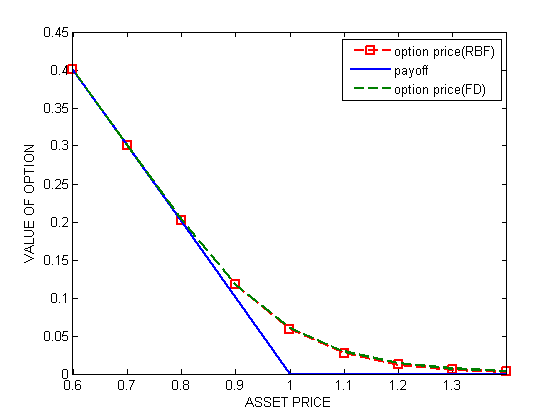
\includegraphics[height=4in]{rbffdpo.png}\
\caption{Comparison between RBF and Finite Difference Solutions }
\vskip -0.5in \vskip -0.5in
\end{centering}
\end{figure}

\begin{table}[h]
\centering
\begin{tabular}{|c|c|c|c|c|c|c|}
  \hline
  % after \\: \hline or \cline{col1-col2} \cline{col3-col4} ...
  S &  Option Value& FD1001  \\
  \hline

  0.6 & 0.4134769 &0.4000037 \\
  0.7 &0.3191524&0.3001161 \\
  0.8 &0.2295821& 0.2020397 \\
  0.9 & 0.1513232&0.1169591  \\
  1.0 & 0.0913208&0.0602833 \\
  1.1 & 0.0513920&0.0293272\\
  1.2 & 0.0277877&0.0140864 \\
  1.3 & 0.0149302 &0.0038609 \\
  1.4& 0.0082378&0.0038609 \\
 \hline
CPUTIME&0.312002&\\
\hline
 RMSE&0.0216&\\
  \hline

\end{tabular}
  \caption{Finite Difference solution at $N=2001,\epsilon=10^{-2},\Delta t=0.1$.}\label{Tab_}
\end{table}

\newpage
\begin{figure}
\begin{centering}
%\vskip -0.5in
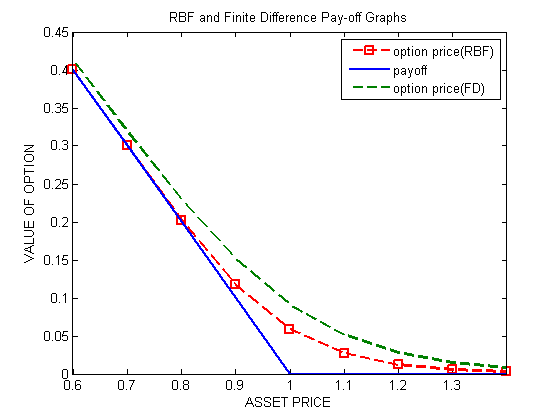
\includegraphics[height=4in]{rbffd101.png}\ \caption{RBF \textit{N}=101, \textit{k}=0.01 and FD
\textit{N}=2001,\textit{k}=0.01 }
 \vskip -0.5in

\end{centering}
\end{figure}

 \begin{figure}[h]
\begin{centering}
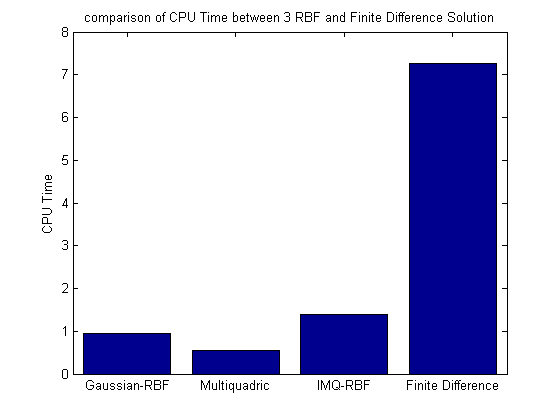
\includegraphics[height=3in]{cpue10000.png}\
\caption{Comparison of CPU Times between the 3 RBFs for $N=101$ and
FD for \textit{N}=2001 } \vskip -0.5in
\end{centering}
\end{figure}

\begin{figure}[h]
\begin{centering}
\vskip -0.5in
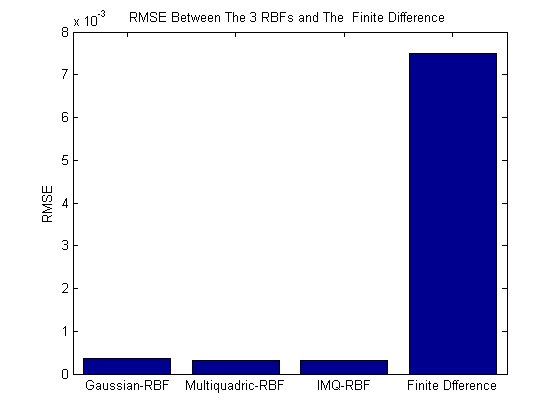
\includegraphics[height=3in]{barrmsee10000.png}\
\caption{Comparison of RMSE between the 3 RBFs for $N=101$ and FD
for \textit{N}=2001 }
\end{centering}
\end{figure}
%-------------------------------------------------------------------------------------------------------------------------
%================================================ Chapter 8  ==============================================================
\sect{\uppercase{Conclusion}}
%-------------------------------------------------------------------------------------------------------------------------




\cleardoublepage

%=================================================BIBLIOGRAPHY==============================================================
\newpage
\begin{center}
{\bf BIBLIOGRAPHY}
\end{center}
\addcontentsline{toc}{section}{\rm BIBLIOGRAPHY \dotfill}
\begin{thebiblio}{99}
%---------------------------------------------------------------------------------------------------------------------------



\bibitem{BS73}
F. Black, M.S. Scholes, \emph{The pricing of options and corporate
liabilities}, Journal of Political Economy 81 (1973) 637-659
\bibitem{Fas02}
G.E. Fasshauer, A.Q.M. Khaliq, D.A. Voss, \emph{Using meshfree
approximation for multi-asset American option problems}, Journal of
Chinese Institute of Engineers, 27 (2004) 563-571

\bibitem{NB11}
N. Flyer and B. Fornberg,\emph{ Radial basis function: Development
and applications to planetary scale flows, Computers and Fluids}
46(2011) 23-32.
\bibitem{BEN11}
B. Fornberg, E. Larsson, and N. Flyer,\emph{ Stable computations
with Gaussian Radial Basis Functions}, SIAM Journal on Scientific
Computing, 33 (2011), 869-892.
\bibitem{YZE07}
Y. Goto, Z. Fei, S.Kan, and E. Kita, \emph{Options valuation by
using radial basis function approximation}, Engineering Analysis
with Boundary Elements, 31(2007) 836-843.
\bibitem{Hon09}
Y.C. Hon and Z. Yang, \emph{Meshless collocation method by
Delta-shaped basis functions for default barrier model}, Engineering
Analysis with Boundary Elements 33(2009) 951-958.
\bibitem{ADS06}
A.Q.M. Khaliq, D.A. Voss, S.H.K. Kazmi,   \emph{A linearly implicit
predictor-corrector scheme for pricing American options using a
penalty method approach}, Journal of Banking and Finance,30 (2006)
489-502.
\bibitem{BSA02}
B. Nielsen, O. Skavhaug, and A. Tveito, \emph{Penalty and
front-fixing methods for the numerical solution of American option
problems}, Journal of Computational Finance, 5 (2002) 69-97.
\bibitem{BOA08}
B. Nielsen, O. Skavhaug, and A. Tveito,\emph{ Penalty methods for
the numerical solution of American multi-asset option problems},
Journal of Computational and Applied Mathematics, 222 (2008) 3-16.
\bibitem{UEG}
U.  Pettersson, E. Larsson, G.  Marcusson, and J. Persson,
\emph{Improved radial basis function methods for multi-dimensional
option pricing}, Journal of Computational and Applied Mathematics,
222 (2008) 82-93
\bibitem{SE09}
S. A. Sarra and E. J. Kansa,  \emph{Multiquadric Radial Basis
Function Approximation Methods for the Numerical Solution of Partial
Differential Equations}. Advances in Computational Mechanics, Tech
Series Press, 2 (2009).
%\bibitem{PSJ}
%Paul Wilmott,Sam Howson,Jeff Dewynne  \emph{The Mathematics of
%Financial Derivatives}. A Student Introduction, Cambridge university
%press.
\bibitem{higham}
Desmond J. Higham  \emph{An Introduction to Financial Option
Valuation}. Mathematics,Stochchastics and Computation,cambridge
univeristy press(2004).
\bibitem{CF}
Omur Ogur \emph{An Introduction to Computational Finance}.Imperial
College press
\bibitem{Wilmot}
Paul Wilmot,Sam Howson,Jeff Dewynne\emph{The Mathematics of
Financial Derivatives}:A Student Introduction.Cambridge University
press
\bibitem{Hon}
Yiu-Chung Hon,Xian-Zhang Mao\emph{A Radial Basis Function Method for
    Solving Options Pricing Models}.The Journal of Finacial
    Engineering.(1999)

\bibitem{KK}
A.Q.M. Khaliq, D.A. Voss,Greg E.Fasshauer\emph{A Parallel Time
Stepping Approach using Mesh-free Approximations for Pricing Options
with Non-Smooth Payouts}:A Student Introduction.The Journal of
Risk(2009)
\end{thebiblio}
%=================================Appendix separation page ===========================================================
\Appendixpage
%---------------------------------------------------------------------------------------------------------------------

%================================================= Appendix A =========================================================
\appen{\uppercase{ Sample Appendix}}\label{app1}
%-------------------------------------------------------------------------------------------------------------------






%=========================Appendix B===================================================================================
\appen{\uppercase{Sample Appendix 2}}\label{app2}
%----------------------------------------------------------------------------------------------------------------------

\subsection{Section Heading} Insert text here.
\subsubsection{Subsection Heading}
\lstinputlisting{tridiagonal.m}

%\lstinputlisting{tridiagonal.m}

%\begin{verbatim}
%function y=lbc(E,T,r,t)
%% Boundary Condition at s=0;
%%Black-Scholes Equation
%%E=1;r=0.1;
%%T=1;
%%***********************************
%% PUT
%% y=E*exp(-r*(T-t));
%%y=E;
%%*************************************
%% CALL
%y=0;
%\end{verbatim}


\end{document}
